
\documentclass[journal]{journal}
\usepackage{fullpage}
\usepackage{url}
\usepackage[margin=1.1in]{geometry}
\usepackage{graphicx}
\usepackage{csvsimple}
\usepackage{varwidth}
\usepackage{array}
\usepackage{float}
\usepackage{amsmath}
\usepackage{pgfplotstable}
\usepackage{amsmath }
\usepackage[T1]{fontenc}
\usepackage[compact]{titlesec}
\usepackage{authblk}

\author[1]{Bernstein Ran}
\author[2]{Shafir Tal}
\author[3]{Tsachor Rachelle}
\author[4]{Studd Karen}
\author[1]{Schuster Assaf}
\affil[1]{Department of Computer Science, Technion I.I.T, Haifa, Israel}
\affil[2]{The Graduate School of Creative Arts Therapies, University of Haifa}
\affil[3]{School of Theatre \& Music, The University of Illinois at Chicago}
\affil[4]{School of Dance, George Mason University}
\hyphenation{op-tical net-works semi-conduc-tor}

\pagestyle{empty}

\begin{document}
\nocite{*}

\title{Laban Movement Analysis using Kinect}

\maketitle
\thispagestyle{empty}


\begin{abstract}
Laban Movement Analysis (LMA), developed in the dance community
over the past seventy years, is an effective method for observing, describing, notating, and interpreting human
movement to enhance communication and expression in everyday and professional life.
Many applications that use motion capture data might be significantly
leveraged if the Laban qualities will be recognized automatically.
This paper presents an automated recognition method of Laban qualities from
motion capture skeletal recordings and it is demonstrated on the output of
Microsoft's Kinect V2 sensor.
\end{abstract}

\begin{IEEEkeywords}
Laban Movement Analysis, Kinect, Machine Learning.
\end{IEEEkeywords}

\IEEEpeerreviewmaketitle



\section{Introduction}

\subsection{Laban movement analysis}
LMA is a formal language for motion description first developed by Rudolf Laban \cite{Laban} and colleagues in the middle of the 20th century. 
LMA describes both conscious and unconscious human movement, based on Laban's categories of \textit{Body}, \textit{Effort}, \textit{Shape}, and \textit{Space}. 
LMA has been used in the fields of dance, acting, athletics, physical therapy, and psychology and behavioral science.
LMA helps actors create momentary moods and portray personality traits through
movement. For example, LMA work investigates the \textit{Effort} properties
\textit{Flow}, \textit{Space}, \textit{Time} and \textit{Weight} of all movement and helps actors 
think specifically about why their character might move in a jerky, fast, light and direct manner 
versus a heavy, slow, indirect and uninterrupted manner.
\begin{figure*}[ht]
\centering
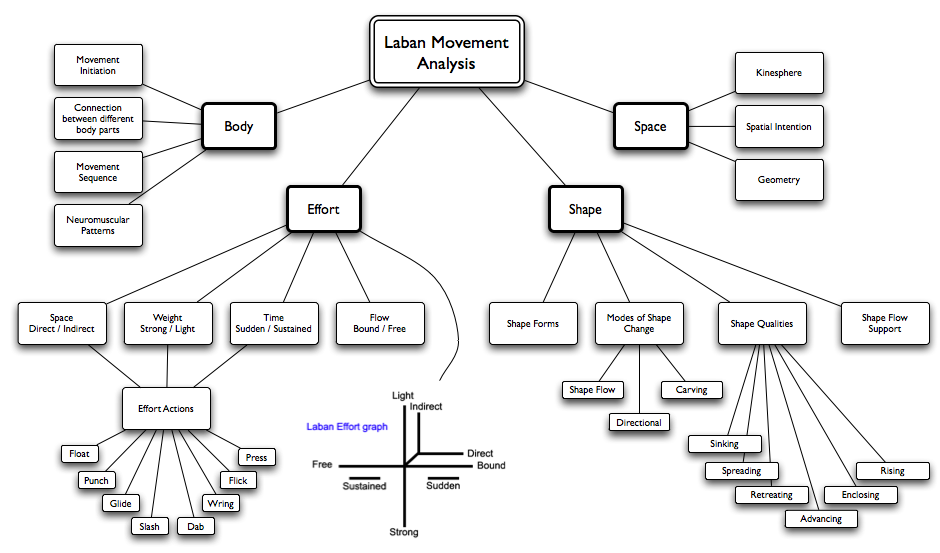
\includegraphics[width=\textwidth]{laban.png}
\caption{Main axes of LMA. Taken from \cite{labanTree}}
\label{labanTree}
\end{figure*}
The entire LMA hierarchy is shown in figure \ref{labanTree}.

\subsection{Motivation for Automated LMA}
There are numerous applications for computerized identification of the qualities that characterize each possible human movement. Examples include the generation and control of specific expressive movements 
of avatars, virtual characters, or robots in mixed reality scenarios
\cite{Masuda}; detection of personality traits during a job interview
\cite{levy2003use}; early detection, severity assessment or revealing of genetic tendency (phenotype) towards various illnesses such as Alzheimer's,
autism, Parkinson's disease \cite{camurri2003application}, or schizophrenia,
based on analysis of the person's motor behavior. Automated emotion recognition from movement is another 
important application, which may have a variety of uses such as online feedback 
to presenters to help them convey through their body language the emotional message they want to communicate 
(e.g., politicians and public speakers or actors in training) \cite{nguyen2012online}; or recognition 
of people's emotions during interactive games such as those played using the Xbox \cite{Zacharatos}. 
\\\\For reducing our data collection and analysis effort, we focused our work on
18 Laban qualities (as listed in Diagram \ref{oneCMAFinal}) that have been found
predictive for emotional state \cite{ShafirPrivate}.

\subsection{Related Work}
Several attempts were made to recognize Laban qualities. The first was Chi et al. \cite{chi2000emote}, who quantified \textit{Effort} and \textit{Shape} for animation. Most of the other attempts were for emotion recognition in the context of Human Robot Interaction (HRI). Martin et al. \cite{martin} analyzed the importance of gestures in emotion recognition for HRI. Masuda et al. generated emotional body motion for a human 
form robot \cite{Masuda}. Rett et al. proposed a human motion recognition 
system using a Bayesian reasoning framework \cite{Rett}. The second line of works focused on LMA (not on emotions), but not using Kinect. Lourens et al. \cite{lourens2010communicating} used video data and Samadani et al.
\cite{samadani2013laban} used a high quality MOCAP camera, but both of them
analyzed only hand gestures. A third line of works used Kinect as the main
sensor for skeletal information. Gabel et al.
\cite{gabel2012full} used Kinect for gait analysis. The work of
Zacharatos et al. \cite{Zacharatos} was inspired by LMA for emotion recognition using Kinect. His feature extraction method was influenced by LMA principles, but he did not attempt to recognize the qualities themselves. Kim et al. \cite{kim} did attempt to do so but not on a real dataset and their work did not include a performance evaluation.
\section{Method}
Because we are the first to handle Laban recognition with
Kinect, we had to create a dataset from scratch. To reduce the noise, and ensure that we capture the essence of the Laban qualities in our dataset, we decided that most of it should be built by recording several Certified [Laban] Movement Analysts (CMA), with just a few validation clips taken from recordings of ordinary people. We did not want to constrain the lengths of the clips to be equal, so in order to get feature vectors of uniform length (regardless of the original length of the clips),
every feature is function of a whole clip (for example, the variability of the
elbow's acceleration). On the uniform length feature vector we applied feature
selection, single task learning (learning a model for every quality separately),
and multitask learning (learning a model for all the qualities together).
\subsection{Clip Collection}
Two main datasets were collected: 
\begin{itemize}
  	\item 
	 CMA dataset - includes 6 CMAs performing in about
	80 clips each (a total of 550 clips). Every clip is about 3 seconds long, and the CMAs executed combinations of the 18 qualities. 
	To achieve uniform distribution of the Laban qualities over the dataset, in every 
	clip the CMA was asked to perform actions that include several specific qualities, 
	and nothing but them.
	
	\begin{figure}[h]
	\centering
	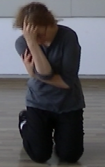
\includegraphics[width=30mm]{Rachelle.png}
	\caption{CMA during a clip}
	\label{Rachelle}
	\end{figure}
	
	\item 
	Non-CMA dataset - includes 2 subjects without a background in movement
	analysis, performing 30 clips each. Every clip is also about 3 seconds long,
	and the subject was asked to perform one out of several
	tasks.
\end{itemize}
\subsection{Clip Labeling}
To achieve a ground truth labeling for the two datasets, every clip was tagged by
a committee of 2 CMAs who determined which Laban qualities appear in the
clip. The use of a committee decision instead of the subjective opinion of one
CMA decreases the labeling noise and the decision is considered as ground truth.
\subsection{Feature Extraction}
Due to the unequal length of clips, all the extracted features are in whole clip 
granularity. We extracted two groups of features, the first is a relatively
small, and contains about 100 features that each one of them is designed for a
specific quality. The second group contains about 6000 features, and exploits the rich data that
is provided by Kinect, by extracting from every joint in the skeleton, the
angular velocity, acceleration, and jerk. For every joint/metric pair, the mean,
variance, skew, and kurtosis were extracted (the extraction of the last four moments is denoted as $\phi$).
\\\\We denote $\vec{P}_{j}(t)$ as the vector (as we get it from the Kinect) of
the position of joint $j$ in time $t$ in a clip with $n$ frames, and
$\alpha_{j}$ is a coefficient proportional to the mass around the joint.
\subsubsection{Shape Analysis: Sagittal Plane}
Laban shape analysis of the sagittal plane is based on the distinction
between two qualities, \textit{Advance} and \textit{Retreat}. This distinction was quantified by projecting the 
velocity vector of the Center of Mass (CM) on the vector of the front of the
body.
The CM was approximated in this case by the average of all the joints. 
The front of the body was approximated by the perpendicular vector to the vector 
between the Left Shoulder (LS) and
the Right Shoulder (RS).
\\\\If $sag$ stands for sagittal, then from the definition of CM of a physical
system,
\\
\\$\vec{P}_{CM}(t) = \sum_{j \in Joints} \alpha_{j}\vec{P}_{j}(t),
\\
\\\vec{P}_{shoulders}(t)=\vec{P}_{LS}(t)-\vec{P}_{RS}(t),$
\\\\the front is perpendicular to $\vec{P}_{shoulders}$, so we can easily calculate it with:
\\\[\vec{P}_{front}=\vec{P}_{shoulders}\left( \begin{array}{ccc}
0 & 0 & 1 \\
0 & 1 & 0 \\
-1 & 0 & 0 \end{array} \right),\]
\\\\$S_{sag}(t) = \vec{P}_{CM}(t)\cdot\vec{P}_{front}(t),$ 
\\\\$\vec{F}_{sag} = \phi([S_{sag}(1), \ldots S_{sag}(n)]),$
\\\\where $\phi$ was denoted in the beginning of the section.
\subsubsection{Shape Analysis: Horizontal Axis}
Here the distinction is between \textit{Spreading} and \textit{Enclosing} on the horizontal axis.
This distinction was quantified by measuring the average distance between every joint to 
the vertical axis of the body that extends from the Head (H) to the Spine Base (SB).
\\
\\$d_{j} = \frac{\left|(\vec{P}_{j}-\vec{P}_{SB})\times
(\vec{P}_{j}-\vec{P}_{H})\right|}{\left|\vec{P}_{H}-\vec{P}_{SB}\right|},
\\
\\S_{horiz}(t) = \sum_{j \in Joints} d_{j}(t),
\\
\\\vec{F}_{horiz} = \phi([S_{horiz}(1), \ldots S_{horiz}(n)]),$
\subsubsection{Shape Analysis: Vertical Axis}
Here the distinction is between \textit{Rise} and \textit{Sink} on the vertical
axis.
This distinction was quantified by measuring the average distance on axis y of each joint from the CM. This quantification is based on the assumption that the body
is ``longer'' when rising.
\\\\$S_{vert}(t) = \sum_{j \in Joints}
\left|\vec{P}_{j}-\vec{P}_{CM}\right|,
\\\\\vec{F}_{vert} = \phi([S_{vert}(1), \ldots S_{vert}(n)]),$
\subsubsection{LMA Effort Analysis: Time Category}
Here the distinction is between \textit{Sudden} and \textit{Sustained}. This quality was quantified by the skew of the acceleration, relying on the assumption that the
acceleration of a sudden movement will be skewed further to the left, i.e., will get
a higher value at the beginning of the movement.
\subsubsection{Effort Analysis: Space Category}
Here the distinction is between \textit{direct} and \textit{Indirect} motion.
This quality was quantified by the angle between the movement vector of a joint to the next one,
relying on the assumption that in direct movement every vector will be in
the same direction as the last (the angle between them is small).
The velocity direction $V$ is calculated by
$\vec{V}_{j}(t) = \vec{P}_{j}(t+1) - \vec{P}_{j}(t),$
and the angles between a direction to the next one is calculated with the inner product
$\vec{A}_{j}(t) = \vec{V}_{j}(t+1) \cdot \vec{V}_{j}(t).$

\subsection{Performance Evaluation}
From a statistical point of view, we have 18 possible labels (Laban qualities) for every clip. 
Each clip was a combination of just a few of these, often 3-4, which means that there is about 
an 85\% chance that a quality won't appear in a clip. Due to this sparsity, accuracy alone is 
not a relevant metric for the performance evaluation because one can get 85\% accuracy by stating 
that for every recording none of the qualities appear. 
A better evaluation would have to combine the precision and recall rates of the classifier. 
This can be done using the F1 score:
\begin{equation*}
F_{1} = \frac{2\cdot precision\cdot recall}{precision+recall}.
\end{equation*} 
\subsection{Feature Selection}
Every clip is extracted into a vector of 6120 features, most of which are noisy or redundant, thus requiring massive feature selection. The feature selection is done in three stages:
	\begin{itemize}
		\item
		Computing the Anova F-value for every feature over the training set. Cross-validation was used to determine the optimal number of features that should be
		left. As seen in Figure  \ref{selection}, filtering out most of the features yielded better          results than not filtering them, where using the top 4\% of features was optimal.
		\begin{figure}[ht!]
			\centering
			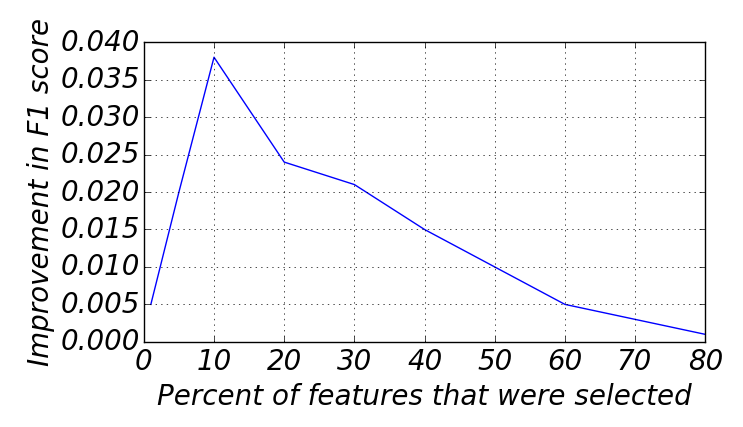
\includegraphics[width=60mm]{featureSelection.png}
			\caption{Influence of the number of features on the performance. The
			selection was made according to statistical significance.
			The blue line is the difference between the score with and without feature
			selection. It can be seen that the optimal fraction of features to select is
			4\%.}
			\label{selection}
			\end{figure}
		\item
			The second phase of feature selection was conducted by Information Gain (IG) rating of the features. As seen in Figure  \ref{igFromFclassif}, the optimal ratio was obtained by selecting the top 60\% out of the features that remained after the first
			phase of feature selection.
			 \begin{figure}[h]
				\centering
				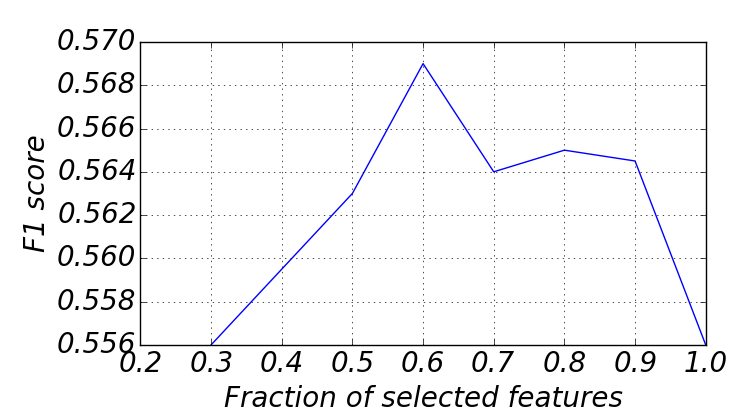
\includegraphics[width=60mm]{igFromFclassif.png}
				\caption{Influence of the number of features selected with IG from the subset
				of features chosen in the first phase on the performance. The
				optimal ratio was 60\%.}
				\label{igFromFclassif}
			\end{figure}
			Examples of qualities and their most significant feature are given in 
			Table \ref{bestFeatures}. The ``Information Gain'' metric used
			in the table is defined as:
			\begin{equation*}
			       IG(T,f) = H(T) - H(T|f),
			\end{equation*}
			where T is the training set, f is a feature, and H() is the information
			entropy of a dataset.
			 \begin{table*}
			   \centering
			   \csvautotabular{rankFeatures.csv}
			   \caption{Example of several qualities and the feature found to be
			   the most informative for them. ``Relative position'' stands for the
			   position of the joint relative to the ancestor joint in the joint
			   hierarchy.}
			   \label{bestFeatures}
			\end{table*}
		\item
		The third phase of feature section was conducted using the Least Absolute Shrinkage and
		Selection Operator (LASSO) regularization.
	\end{itemize}

\section{Experimental Setups and Results}
\subsection{Multilabel Classification}
Multilabel learning deals with the problem where each instance is associated
with multiple labels simultaneously, where the number of labels is not fixed
from instance to instance. The task of this learning paradigm is to predict
the label (Laban quality) set for each unseen instance (skeletal recording), 
by analyzing training instances with known label sets. The multilabel
approach taken in this paper is to break the LMA problem into 18
binary classification tasks --- one for every Laban quality --- where every binary
decision is whether or not the quality exists.
\\The following subsections will describe several experimental setups
where the results in each will serve as a baseline for the next.
\subsection{Per CMA Evaluation}
	In this experiment the train and test datasets are taken from the same
	CMA. The performance on every Laban quality separately 	is demonstrated on 
	a dataset of one of the CMAs in Figure \ref{oneCMAFinal}.
	In Figure \ref{oneCMASummary} the incremental evolution of the algorithm is 
	described from step to step with the next notation:
	\begin{itemize}
	\item 
	\textit{Chance} stands for randomly tossing a balanced coin in every
	classification decision.
	\item 
	\textit{NN} stands for applying the Nearest Neighbors algorithm.
	\item 
	\textit{LinearSVC} stands for Support Vector Classifier (SVC) with a linear
	kernel.
	\item 
	\textit{LabelBalancing} stands for giving greater weight to clips that
	contain the quality due to the small fraction of them in the whole
	dataset.
	\item 
	\textit{Lasso}, \textit{SFS} (Statistical Feature Selection), and \textit{InfoGain} 
	(information gain based feature selection) were described in the
	\textit{Feature Selection} section.
	\end{itemize}

\pgfplotstableread{
x         y    y-max  y-min
Chance          0.23 0.005 0.005
NN              0.26 0.025 0.025
LinearSVC       0.37 0.02  0.02
LabelBalancing  0.41 0.025 0.025
Lasso           0.44 0.025 0.025
SFS             0.48 0.045 0.045
InfoGain        0.53 0.045 0.045
}{\mytable}

\begin{figure}[ht]
\centering   
\begin{tikzpicture}
\begin{axis} [
    width=5cm,
    ymin=0.2,
    ylabel={F1 score},
    symbolic x coords={Chance,NN,LinearSVC,LabelBalancing,Lasso,SFS,InfoGain},
    xtick=data,
    x tick label style={rotate=90,anchor=east}
]
\addplot [ybar, fill=blue!50] 
  plot [error bars/.cd, y dir=both, y explicit]
  table [y error plus=y-max, y error minus=y-min] {\mytable};
\end{axis} 
\end{tikzpicture}
\caption{Evaluation of every CMA's dataset separately in the single task learning
		setting. Each column represents an additional step in the algorithm's evolution.
		The results are the average F1 score and its standard deviation (STD) between the CMAs.}
\label{oneCMASummary}
\end{figure}

\begin{figure*}
	\centering
	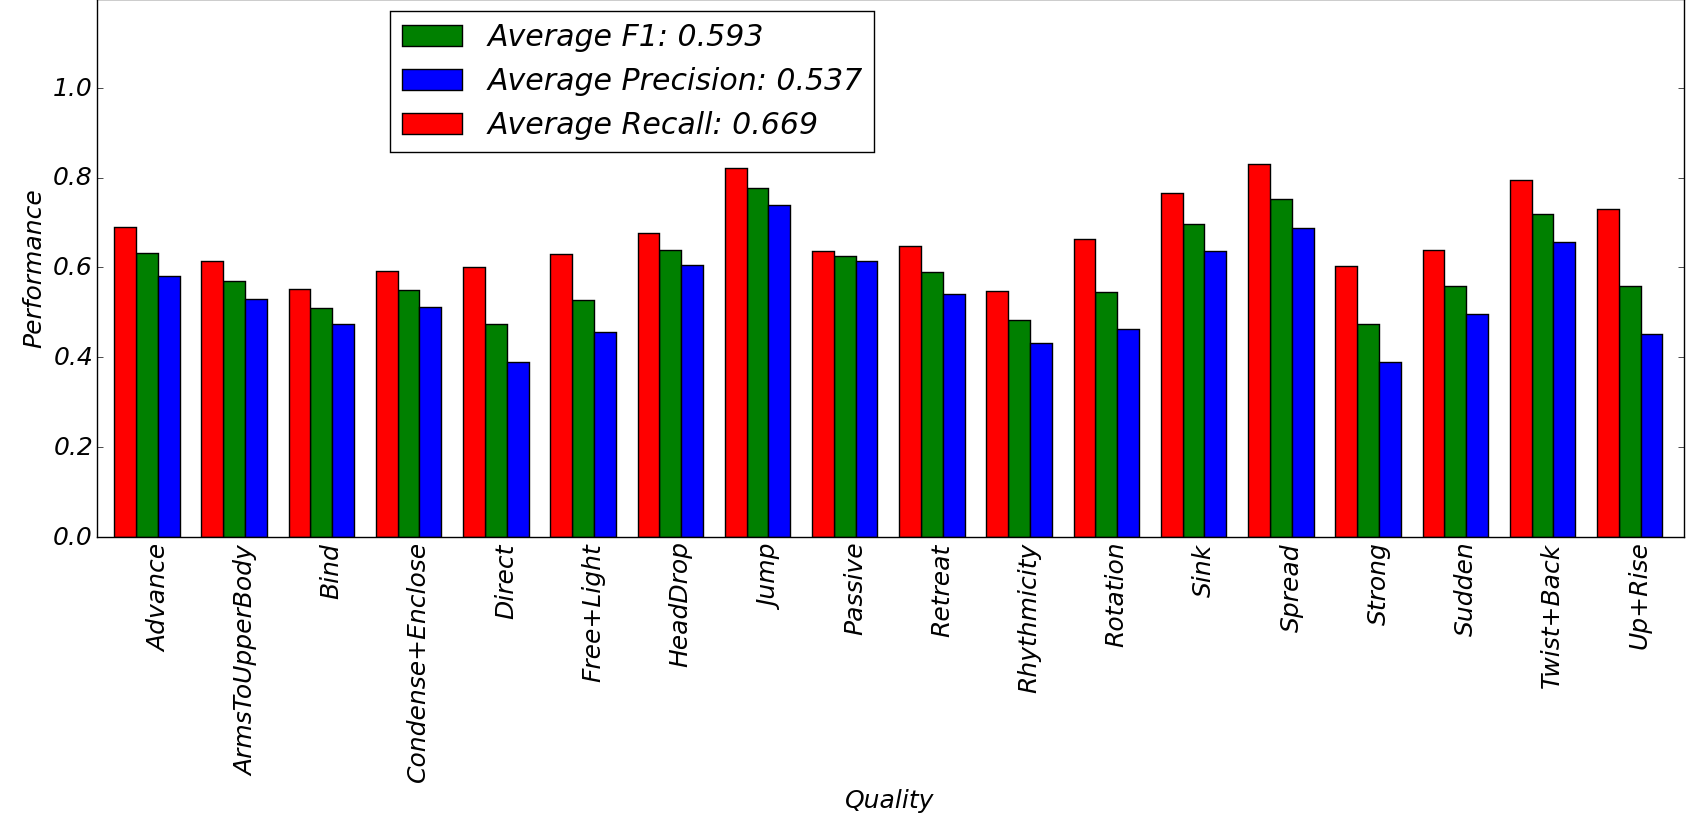
\includegraphics[width=\textwidth, height=60mm]{oneCMAFinalWithoutTitle.png}
	\caption{Recall, precision and F1 score of each Laban quality separately. The
	evaluation was conducted on a dataset that was captured on only one CMA.}
	\label{oneCMAFinal}
\end{figure*}

\section{Conclusion}


\bibliographystyle{unsrt}
\bibliography{bib}

\end{document}


